\documentclass[usegeometry=true]{scrartcl}
 \usepackage{csquotes}
\usepackage[ngerman]{babel}
\usepackage[T1]{fontenc}
\usepackage{lmodern}
\usepackage[utf8]{inputenc}
\usepackage{hyperref}
\usepackage{amssymb}

% Dimensionen bitte nicht ändern. 
\usepackage[left=2cm, right=2cm, top=2cm, bottom=2cm, bindingoffset=1cm, includeheadfoot]{geometry}
%Zeilenabstand bitte nicht ändern
\usepackage[onehalfspacing]{setspace}
\usepackage{graphicx}
\usepackage[backend=biber,style=numeric,]{biblatex}\addbibresource{literatur.bib}

\begin{document}
% ----------------------------------------------------------------------------
\subject{Projektbericht zum Modul Information Retrieval und Visualisierung Sommersemester 2023}
\title{Visualisierungen zur Analyse von Einflussfaktoren auf die Schlaff Effizienz}
%\subtitle{Untertitel}% optional
\author{Mick Stewart Wörner}% obligatorisch
%\date{10.9.2023}
\maketitle% verwendet die zuvor gemachte Angaben zur Gestaltung eines Titels
% ----------------------------------------------------------------------------
% Inhaltsverzeichnis:
%\tableofcontents
% ----------------------------------------------------------------------------
% Gliederung und Text:
\newpage
\section{Einleitung}
Tipps zu Latex und Koma-Script für Hausarbeiten sind im \href{http://mirrors.ctan.org/info/latex-refsheet/LaTeX_RefSheet.pdf}{LaTeX Reference Sheet for a thesis with KOMA-Script} von Marion Lammarsch und Elke Schubert zusammengefasst. 
Der Bericht fällt in die Kategorie von InfoVis-Paper, die Tamara Munzner Design Study nennt ~\cite{Munzner2008}: In der Einleitung sollen sie zuerst das Zielproblem beschrieben. Daraus sollen sie Fragestellungen motivieren, die mittels Techniken der Informationsvisualisierung beantwortet werden können. In dem Abschnitt direkt unter der Überschrift Einleitung sollen Sie nach einer kurzen Einleitung Fragestellungen und das Zielproblem motivieren und besschreiben. 

\subsection{Anwendungshintergrund}

\subsection{Zielgruppen}

\cite*[The association between sleep quality and quality of life: a population-based study Sujin Lee a , Ji Hyun Kim c , Jae Ho Chung b, ]{2}


Die Schlafqualität spielt eine entscheidende Rolle für die Lebensqualität, deswegen richtet sich die Anwendung 
an eine Zielgruppe, die ein Interesse daran hat, die Zusammenhänge und Einflüsse auf die Schlafqualität zu verstehen.
 Diese Zielgruppe könnte aus Forschern und Privatpersonen bestehen, die daran interessiert sind, wie verschiedene 
 Lebensstile die Schlafqualität beeinflussen können und die Schlafzyklen sich zueinander Verhalten.
 Ein tiefgehendes Wissen über die Schlafphasen ist nicht erforderlich, aber ein generelles Interesse an der Analyse des Zusammenhangs zwischen Verhalten und Schlafqualität charakterisiert den Benutzer.
 Die Benutzer sollten sich darüber im Klaren sein, dass die Visualisierungen Hinweise liefern können, 
 jedoch nicht notwendigerweise kausale Zusammenhänge zeigen.

Die Visualisierungen, die in diesem Projekt präsentiert werden, sollen dabei helfen, Einflüsse und Zusammenhänge
 bei der Schlafqualität zu identifizieren. Dabei werden verschiedene Attribute wie Koffein-, Alkohol- und Tabakkonsum
 , Sport, sowie Alter und Geschlecht der Personen untersucht. Die Zielgruppe sollte ein Grundverständnis
  für die Bedeutung dieser Attribute in Bezug auf die Schlafqualität haben.

Die Benutzer sollten sich bewusst sein, dass der Datensatz, der in dieser Anwendung verwendet wird,
 nur 452 Personen umfasst und durch die Datenverarbeitung weiter reduziert wird. 
 Daher ist es wichtig, die statistische Validität der Ergebnisse zu berücksichtigen,
  insbesondere bei der Anwendung von Filtern. Statistische Aussagekraft ist bei n <30 nicht mehr gegeben,
   und daher müssen die Benutzer dies bei der Benutzung berücksichtigen.



\subsection{Überblick und Beiträge}
Im diesem Abschnitt wird eine Überblick auf die Daten und verwendeten Visualisierungstechniken gegeben. 

\section{Daten}

Der verwendete Datensatz bietet eine umfangreiche Sammlung von 15 Attributen, die Informationen 
über die Schlafqualität und Lebensgewohnheiten von 452 Personen liefern.
Auf der Kaggle Seite wird nach Angaben des Authors behauptet, dass der Datensatz im Kontext einer Studie von der ENSIAS, Marroco gesammelt wurde.
Innerhalb einer Literatur Recherche konnten weder auf der Webseite der ENSIAS noch in weitergehender Literaturrecherche eine Veröffentlichung zu diesem Datensatz identifizieren.
Daher sollten die Daten und daraus entwickelten Ergebnisse, nicht unreflektiert übernommen werden. 

Der Datensatz hat drei Nominale (Id, Gender und Raucher) und zwölf Quantitative (Age, Bedtime, Wakeup Time, Sleep Duration, Sleep Efficiency, REM Sleep percentage, Deep Sleep Percentage, Light Sleep Percentage, Awakenings, Caffeine Intake,Alkohol Intake, Tobako Intake, Exercise frequency) Aufgrund der unklaren Herrkunft des Datensatzes muss werden die Attribute im folgenden näher beschrieben.\\
\begin{itemize}
  \item ID: Die ID identifiziert eine Person eindeutig. Da keine ID mehrfach aufgeführt wurde, ist anzunehmen, dass jede Person nur einmal an der Studie teilgenommen hat. Die ID wird als Integer bereitgestellt, und der Datenbereich reicht von 1 bis 452.
  \item Age: Gibt das Alter an, das die Person zum Zeitpunkt der Erfassung hatte. Das Alter wird als Integer angegeben und ist daher diskret, zum Beispiel 43 Jahre. Die Verteilung des Datenbereichs wird im Folgenden in diesem Format angegeben: (Quantile [Min, 25, 50, 75, Max]), Quantile [9, 29, 40, 52, 69].
  \item Gender: Das Geschlecht wird als String abgespeichert und nimmt nur zwei Werte an: ''Male'' oder ''Female''. Dabei gibt es einen Anteil von 50 Prozent Männern und 50 Prozent Frauen.
  \item Bedtime: Gibt die Uhrzeit an, zu der die Person ins Bett gegangen ist. Hierbei ist nicht klar, ob damit der Zeitpunkt gemeint ist, zu dem die Person eingeschlafen ist oder zu dem die Person sich ins Bett gelegt hat. Die Information werden als DateTime angegeben. Die Daten steigen in 30 Minuten schritten und ist trotz DateTime Formati damit Diskret. 
\item WakeUp time = Gibt das Datum und die Uhrzeit an zu dem die Person erwacht steigt analog zu der Bedtime in halben Stunden Schritten an. Das Datum ist bei beiden DateTime formaten nicht von weiterem interesse, da es keine zeitliche Entwicklung der erfassten Personen gibt. 
\item Sleep Duration: Die Schlafdauer ist wie die Bed Time unklar in Ihrer interpretation, da sich der Wert immer aus der Differenz zwischen bedtime und WakeupTime berechnet. Daher ist unklar ob es sich um die geschlafene oder um die im Bett verbrachte Zeit handelt. Die Spalte wird als Float angegeben und steigt aufgrund der halbstündlichen Sprünge der BedTime und WakeupTime auch in 0.5 Schritten. Die Daten haben Quantile von [5.0, 7.0, 7.5, 8.0, 10.0] Stunden.
Die Interprettation der Sleep Duration wird weiter dadurch erschwert, dass im weiterem Datensatz die Anzahl angegeben wird wie oft eine Person in der Nacht wach wird. Aber ohne Anganbe wie lange diese "Schlafpausen" spezifisch sind. 
\item Sleep efficiency = Gibt den prozentualen Anteil an, die eine Person Schlafend im Bett verbracht hat. Die Daten werden als Float mit zwei Nachkommastellen angeben. Die Daten haben die Quantile: [0.5, 0.7, 0.82, 0.9, 0.99]. Eine Person die 5 Stunden im Bett verbracht hat und davon eine Stunde wach war. Hat also eine Schlafeffizienz von 80 Prozent. Da hier wieder eine Interpetations Problematik besteht. Wird im weiteren davon ausgegangen, dass die Schlafeffizienz angibt welchen Anteil die Person nach erstmaligem einschlafen, Schlafend verbingen. Weiter wird diese Kennzahl in der Datenverarbeitung auf einen absoluten Studenwert hoch gerechnet.
\item REM Sleep percentage = Die REM steht für Rapid Eye Movement Schlaf, dies ist einer der drei Schlafzyklen die ein Mensch im Schlaf durchführt. Die CDC empfiehlt einen Anteil von 25 Prozent  \href{https://www.healthline.com/health/how-much-deep-sleep-do-you-need}{Healthline} sollte.  Der REM Percentage gibt den Prozentualen Anteil an den die schlafende Person im REM Verbracht hat. Also Anteil REM an Schlaff Effizienz. Die Daten werden als Integer abgespeichert und haben Quantile von [15, 20, 22, 25 30]  Weiter wird diese Kennzahl in der Datenverarbeitung auf einen absoluten Studenwert hoch gerechnet.
\item Deep sleep percentage? = Der Tiefschlaf Prozentsatzt gibt den  Anteil am Schlaf an, der im Tiefschlaf verbracht wurde. Die Daten werden als Integer angegeben und haben Quantile:[18, 51, 58, 63, 75]  Weiter wird diese Kennzahl in der Datenverarbeitung auf einen absoluten Studenwert hoch gerechnet.
\item Light sleep percentage = Gibt den Prozentualen Anteil am Schlaf an, der im Leichtschlaf verbracht wurde. Die Daten werden als Integer angegeben und haben Quantile von [7, 15, 18, 40, 63] Weiter wird diese Kennzahl in der Datenverarbeitung auf einen absoluten Studenwert hoch gerechnet.
\item Awakenings = Gibt die absolute Anzahl an, wie oft eine Person aufgewacht ist. Die Daten werden im Datensatz als Float abgespeichert. 0.0 bedeutet eine Person hat durchgeschlafen und ist nur einmal Final am morgen aufgewacht. Die Daten reichen von  [0.0, 1.0, 1.0, 3.0, 4.0]
\item Caffeine intake = Gibt an wie viel Koffeein die Person in den letzten 24 Stunden zu sich genommen hat. Die Maßeinheit hierbei beträgt mg. Die Daten werden als Float abgespeichert und haben Quantile von  [0.0, 0.0, 25.0, 50.0, 200.0].
\item Alcohol intake = Gibt an wie viel Alkohol die Personen ind en letzten 24 Stunden zu sich genommen hat in Oz. Die Daten haben Quantile von [0.0, 0.0, 0.0, 2.0, 5.0]
\item Tobacco intake = Gibt an ob die Person Raucht. Die Daten sind als String abgespeichert: Yes für Raucher und No für Nichtgeraucht. 154 Personen geben an zu Rauchen und 298 geben an NichtRaucher zu sein. 
\item Exercise frequency = Gibt an wie viele Einheiten Sport die Person in der Woche macht. Dabei ist nicht angeben welche Maßeinheit diese Einheiten Sport haben. Die Daten haben Quantile von [0, 0, 2, 3, 5], es gibt 6 fehlende Werte. 
\end{itemize}
\textbf{Bei Annahme, dass die Daten legitim sind und die  angegebene Interpettation der Attribute korrekt ist, ermöglicht dieser Datensatz geneu Einblicke in die Schlafqualität vorallem die Schlafphasen und Dauer dieser. Zusätzlich werden relevante Verhaltsweisen und Einflüsse erfasst. Die Erfassung der Einnahme von Kaffee und Alkohol ist, suboptimal, da die beiden Substanzen innerhalb des im menschlichen Körpers eine geringe Halbwertszeit aufweisen. Dahingehend wäre der Zeitpunkt der Einnahme relevant. Weitere Faktoren die die Schlafqualität beinflussen werden nicht erfasst weiter werden die länge der individuellen Schlafunterbrechungen nicht differenziert und den drei Schlafphasen nicht zugeordnet. So könnte es für den Anwender von Interesse zu sein, welche der Schlafphasen durch welche Verhaltensweisen gestört werden. Weiter lässt sich argumentiern, dass die Verteilung der Verhaltensweisen sehr linksseitig ist. Dies mag auf kulturelle Unterschiede zurückzuführen sein. Daher muss die Aussagekräftigkeit des Datensatzen auf den Marrokanischen Lebensstil eingeschränkt werden.}

\textbf{ Die Daten }
Der Datensatz wurde auf  \href{https://www.kaggle.com/datasets/equilibriumm/sleep-efficiency/data}{Kaggle} 
veröffentlicht und unterliegem keinem Copyright Schutz. Die Daten sind als CSV mit einer Größe von 9kB zugänglich.
Die Daten sind in dem Github Repository abgepeichert, dies ermöglicht eine zentrale aktualisierung der Daten, falls dies Nötig sein sollte.  
 Das Programm ruft die CVS Datei  mittels eines Http.get request auf und speichert diese als einen String ab.  
Falls der requst klappt wird die Message `Got Text Ok fulltext' an die Funktion `update' gesendet. Der String ist hierbei repräsentiert durch `fullText'.
Daraufhin wird im `Model' das `datenladen' auf Success gesetzt.
 Auf den String wird die Funktion `stringtoUnverarbeitete', deren Ziel es ist den String in eine List(UnverarbeiteteDaten) zu transformieren.
 Die Funktion benutzt das  Paket BrianHicks/elm-csv (Im Code als Decode)  Diese zieht die Namen der Felder aus der ersten Reihe in dem String. Die Funktion decode decodiert die Inputdaten, relevant hierbei ist das, auch leere Felder in dem String vorkommen dürfen. Die Funktion Decode.blank gibt ein  `Nothing' zurück, falls das Feld leer sein sollte.
 Wenn es doch zu einem Fehler kommen sollte gibt die Funktion stringtoUnverarbeitete eine leere Liste zurück an das Modell.
 Wenn die Daten nun in der Form Unverarbeitete Daten sind wird die Funktion `sleep2Point' angewandt. Diese entfernt einen Tupel, wenn eines seiner Felder ein `Nothing' beinhaltet. Weiter werden die Werte für REM, Tiefschlaf und Leitschlaf in wirklich in diesen verbrachten Stunden transformiert indem diese, 
 mit 0.1 in Prozente übertragen wurden und dann mit der Schlafeffizienz und Schlandauer multipliziert.
 Dies ist besser, da somit die interpretation erleichtert wird, und die Vergleichbarkeit wird hergestellt. Vor der Transformation waren die Schlafphasen einer Person die 5 Stunden schläft und einer Person die 10 Stunden schläft nicht unterscheidbar. Jetzt läsäst sich klar anzeigen wie viel die Personen in den Schlafphasen verbracht haben.
 Gender und Raucher werden von einem String zu einem Float mittels case handeling konvertiert (genderToFloat und raucherToFloat). Dies ermöglicht es mit den Daten zu rechnen und erleichtert das weiter visualisieren. 
 Die Funktion sleep2Point hat einen Output von Typ Alias `Aussortierte Daten'.
 Weiter werden die Attribute Bedtime und Wakeuptime in den aktuellen Visualisierungen nicht benutzt, könnte es bei der Weiterentwicklung interessant werden, daher wurden Sie im Datenkonstrukt belassen aber nicht weiter behandelt. Man könnte von einer sanften Projektion sprechen.
 Innerhalb der Einstellungen kann der Anwender eine Selektion durchführen und Einschränkungen auf das zu untersuchende Attribut anwenden.
  So werden nur Datentupel an die Visualisierungen übergeben die dem Kriterium entsprechen.


   
\newpage
\section{Visualisierungen}
\subsection{Analyse der Anwendungsaufgaben}
Die Aufgaben die durch die Visualisierung gelöst werden sollen: \\ 
 Die Hauptaufgabe der visualisierungen ist es dem Nutzer dabei behilflich zu sein sich 
einen Überblick über die gegebenen Daten zu machen, und die Attribute auf Ihren zusammenhang zu anderen
zu analysieren und dann die größe der Einflüsse der Verhaltensweisen auf das untersuchte Attrbiut zu differenzieren. 
Der Anwender muss zunächst die Datenlage kritisch analysieren und die güte der einzelnen Attribute auf Ihre Aussagekräftigkeit zu bewerten. 
Nach Bewertung der Attribute vergleicht er diese mit anderen Attributen und kann so komplexe Zusammenhänge und Beziehungen erkennen. 
Daraufhin müssen die Einflüsse des Verhaltens auf die Attribute analysiert werden.
Dabei muss der Anwender die Grundlagen der statistischen Interpretation und relevanz
von Normalverteilungen für die Interpretation von Datenlagen kennen. Er sollte also wissen, dass die Datenlage normalverteilt sein sollte, um statistische Aussagen treffen zu können.
Weiter ist es von Nutzen die Korrelation interpretieren zu können. 
Die Interpreatation von Rot als negative und Grün als positive ist von Nutzen um die ergebnisse schneller zu erfassen, ist allerdings nicht notwendig.
\\
\\
Das Problem ist folgendes: Daher ist es wichtig, 
 dass wir die Daten visualisieren um die Zusammenhänge zu erkennen.
Die Visualisierung soll uns also erlauben den Einfluss von multiplen Verhaltensindikatoren auf die Ausprägung eines Merkmales zu schätzen.
\\
\\
Analysieren sie die konkreten Anwendungsaufgaben, die die Lösung des Zielproblems durch die Anwender:innen bearbeitet werden müssen. 

Welche sinnvollen mentale Modelle helfen den Personen bei der Bearbeitung. 
Aufgabenstellung: Analyse der Variablen und den Einfuss der Verhaltensindikatoren
%Welche Visualisierungen helfen den Personen, die die Software verwenden, sinnvolle mentale Modelle aufzubauen. 
Handelt sich um explorative Visualisierung 
Menatle Modelle: Was ist eine Normalverteilung? 
Abweichungen von der Linie:
  Ein Verständnis dafür, wie Abweichungen von der diagonalen Linie im QQ-Plot auf nicht-normale Verteilungen oder systematische Abweichungen hinweisen können.
  Schwänze und Spitzen:
Das mentale Modell von Schwänzen und Spitzen in einer Verteilung hilft dabei zu verstehen, wie sich Ausreißer oder starke Konzentrationen von Werten auf den QQ-Plot auswirken können.
\\
\\

Sind diese mentalen Modelle für sie notwendig, um die Aufgaben lösen zu können? 
Gehen sie bei ihrer Argumentation von den Anwendungsaufgaben aus und kommen sie dann zu den mentalen Modellen, deren Aufbau durch Visualisierungen unterstützt wird. 
\subsection{Anforderungen an die Visualisierungen}
Leiten sie Anforderungen an das Design der Visualisierungen ab, die sich durch ihre Analyse des Zielproblems ergeben.

\textbf{ Anforderungen an das Design. }
\subsection{Präsentation der Visualisierungen}






\subsubsection{Visualisierung Eins: QQ-Plot Datenlage Normalverteilt?}

Die erste Visualsierung ist die Darstellung der Daten in einem Scatterplott. Spezifisch der eines Normalverteilung QQ Plots. 
Ein QQ-Plot (Quantile-Quantile-Plot) ist ein nützliches grafisches Werkzeug in der statistischen Datenanalyse, insbesondere wenn es darum geht, die Verteilung von Daten zu überprüfen und mit einer theoretischen Verteilung zu vergleichen, in der Anwendung wird, Aufgrund des Implementationaufwandes, nur der vergleich mit der Normalverteilung vorgenommen. 
Die Visualisierung zeigt den Wert auf der Y achse an, den ein Datenpunkt hätte, falls der Datensatz einer Normalverteilung folgen würde.
Diese werden dann auf einem zwei dimensionalem Diagramm dargestellt. Die X Achse zeigt die Quantile der Daten an, die Y Achse zeigt die Quantile der Normalverteilung an.

Die Typischen Aufgabenfelder eines QQ Plots sind die Normalitätsüberprüfung, die Identifikation von Abweichungen, die Bestätigung der Normalverteilungshypothese und Identifikation von Ausreißern.
Bei der Normalitätsüberprüfung, der primäre Zweck eines QQ-Plots, geht es darum zu überprüfen ob ein Attribut 
einer Normalverteilung folgt. Ein perfekter QQ-Plot würde alle Punkte auf der Linie der Gleichverteilung platzieren.
 Abweichungen von dieser Linie deuten auf Abweichungen von der Normalverteilung hin. Der Anwender kann in der Visualisierung
 sehen ob die Attribute einer Normalverteilung folgen. Falls diese Perfekt Normalverteilt sein sollten, liegen die Datenpunkte 
 direkt auf der schwarzen Linie. Die in der Grafik eingezeichnete rote Line ist vom 25 Quantil bis zum 75 Quantil gezogen. Dies lässt den Anwender überprüfen ob es eine additive verschiebung gibt. 
Die Identifikation von Ausreisern, können im Normal QQ-Plot, an den visuellen Enden identifiziert werden. Starke abweichungen sind durch eine große Distanz zur schwarzen Linie identifizierbar. Diese können durch das Filtern des Datenbereiches entfernt werden. 
weiter ist es möglich einen Vergleich verschiedener Verteilungena anzustellen. Dies ist aufgrund des Umfang des Projektes nicht in der Anwendung implementiert
Dies Ermöglicht es dem Anwender die Daten und interpretierbarkeit einzuschätzen und diese in geringem Maße mit den Filtern zu Selektieren. Dies erlaubt es dem Anwender die aussagekräftigen Attribute von den aussageschwachen zu unterscheiden.


\begin{figure}[h]
  \centering
  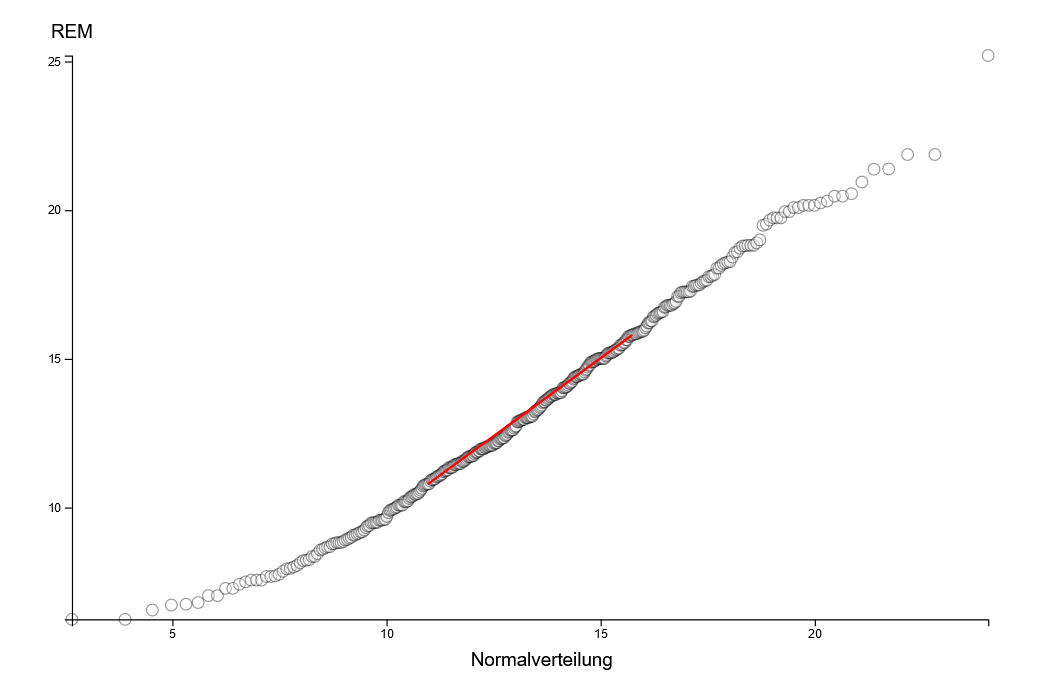
\includegraphics [width = 0.8\textwidth]{NormQQPlott.JPG}
  \caption{Visualisierung Eins  Norm QQ-Plot REM }
\end{figure}

Das oben Auswählen und das Filtern geschieht in der Seitenleiste, hier kann der Benutzer das Atrribut auswählen, dass er untersuchen möchte und direkt darunter dieses in seinem Wertebereich filtern. 
Der eingeschränkte Datenbereich wird dann in den anderen Visualisierungen verwendet.
Der Benutzer kann in der zweiten Visualisierung zwei weitere Attribute zum untersuchen auswählen. Diese werden darufhin unter dem Hauptscatterplott als kleinere QQ-Plott dargestellt und ermöglichen eine schnelle Einschätzung der Güte. 
Hier mit wird vissualisiert, dass die Attribute mit denen verglichen wird den gleichen Ansprüchen gegenüberstehen muss wie das Hauptattribut.


Alternativ hätte auch ein Histogramm verwendetwerden können, bei diesel hätte ein Distributionfitting leichter stattfinden können. 
\\

Expressivität und Effektivität der Visualisierung diskutieren.\\

Die Zielgruppe der Visualisierungen sind Nutzer mit einem Interesse an den zu grundeliegenden Daten. 







\subsubsection{Visualisierung Zwei: Parallele Koordinaten}
Präsentieren der Visualisierung und Interaktionsmöglichkeiten. 
3 Dimensionen werden abgebildet. Die in QQ-Plott ausgewählte sowie zwei Weitere Atrribute. Die Achsen sind Parallel zueinander angelegt und gleich groß. Die Ausprägungen eines Datupels werden dargestellt, indem man die Ausprägung den der Tupel am Attribut hat auf die Y achse Skaliert. Dann wird eine gerade linie zwischen den positionen auf den anliegenden Achsen gezogen. 
Die Endpunkte der Liniensegmente korrespondieren also mit den Attributwerten.
Das Hauptattribut, welches in Visualisierung 1. ausgewählt wurde ist in der Mitte anglegegt. Das Y Attribut zu der linken und das Z Attribut zu der rechten Seite.
Es wurde bewusst darauf verzichtet weitere Attributsdimensionen hinzuzufügen, da es einerseits der Anwender einen Fokus auf die Analyse des Hauptattributes hat und andererseits, bei mehr als 3 Attributen zusammenhänge suggeriert werden könnten, die nicht unbedingt vorhanden sein müssen. Nur weil eine Clusterung zwischen Dimension 1 und 2 und zwischen 2 und 3 beseteht. Bedueted das nicht immer, dass es eine Clusterung zwischen 1 und 3 gibt. 
 Dies ist der Effektivität abträglich, da so zusammenhänge suggeriert werden könnten di enicht intendiert sind.

Die Parallelen Koordinaten eignen sich gut für mehrdimensionale, quantitative und endliche Daten. 
(Dimension< 20)


\begin{figure}[h]
  \centering
  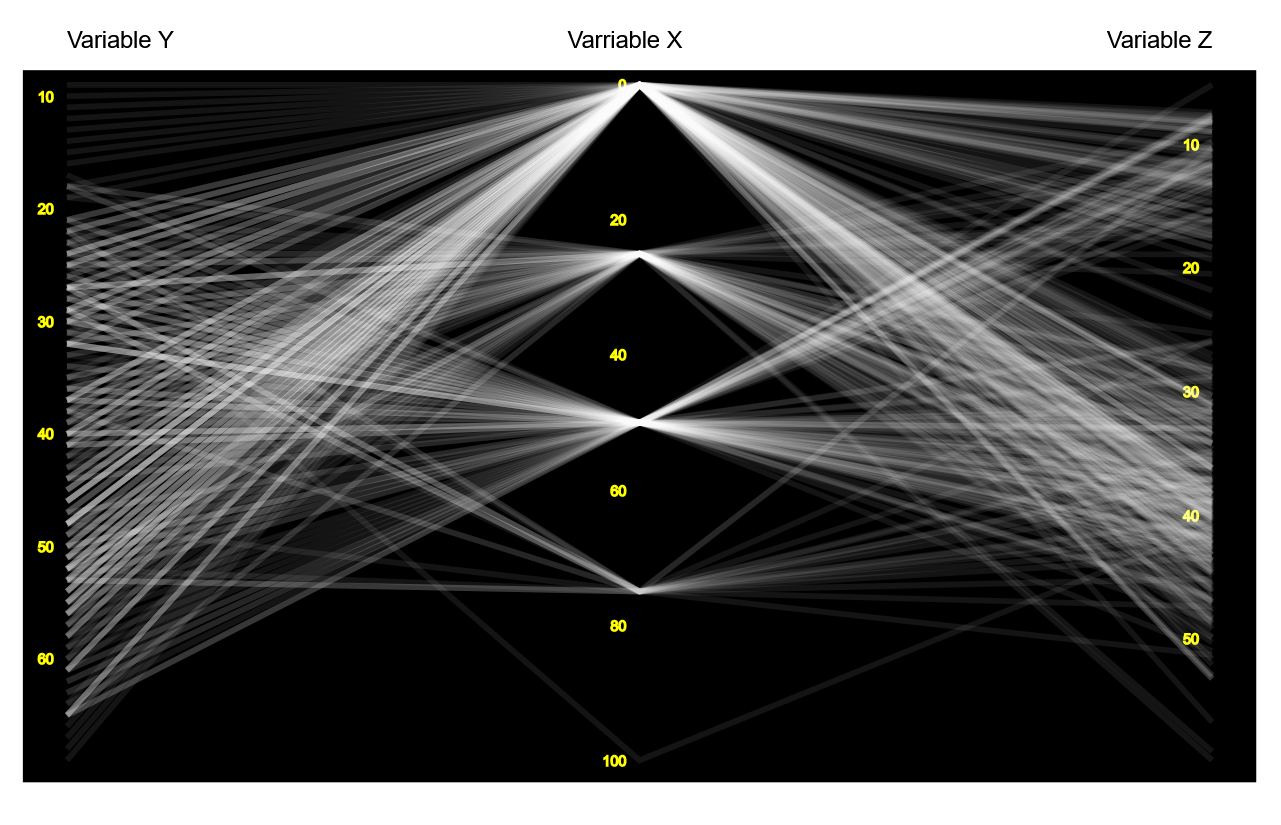
\includegraphics [width = 0.8\textwidth]{RoengtenBSP.JPG}
  \caption{Visualisierung Eins  Norm QQ-Plot REM }
\end{figure}

Wieso sind diese gut und erfüllen die Anforderungen an das Design?



Wieso erfüllt die Visualisierung den Anforderungen der Anwender?

 Der Anwender hat ein Interesse die Zusammenhänge zwischen dem Hauptattribut und den anderen Attributen zu untersuchen, die nicht leicht mit statsitischen Test erkannt werden können.
  Durch die Betrachtung der Linien können Muster, Trends oder Gruppierungen in den Daten identifiziert werden, die auf Beziehungen zwischen den attributen Hinweisen.
  Zum Beispiel können parallele Linien auf eine starke Korrelation zwischen den entsprechenden Variablen hinweisen. 
  Der Anwender kann somit Rückschlüsse auf den zusammenhang von Attributen ausbilden und diese mithilfe von Visualisierung NR. 3 
  Rückschlüsse auf die, hinterden Daten liegenden Mechanismen schließen und somit sein Verständnis von Schlafqualität zu verbessern.
 Die Untersuchung der Attribute und das Visualisieren kann mittels eines interaktiven anpassens der Pixelgröße und RGBA Werte erfolgen, dies ist vorallem nützlich, da viele der Inputdaten wenige unterschiedliche Wertausprägungen haben, was die Clusterung der Inputdaten erschwert. Um dennoch interessante Muster erkennen kann. So kann der Benutzer basierend auf seinen eigenen visuellen Bedürfnissen anpassungen vornehmen. In Bild 3 wird dies vorgestellt.
 
\begin{figure}[h]
  \centering
  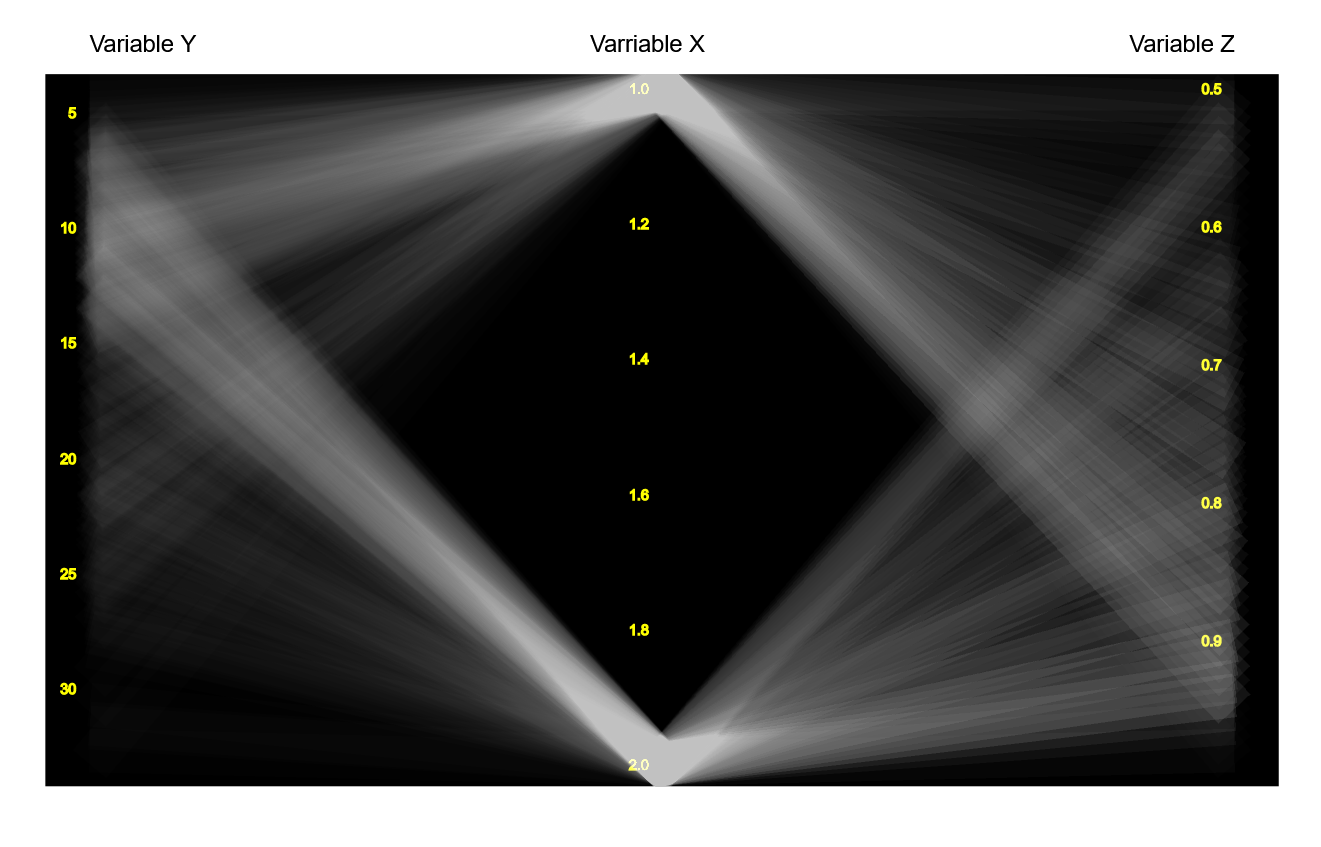
\includegraphics [width = 0.8\textwidth]{ParalleleBSPPixel.JPG}
  \caption{Visualisierung Zwei: Parallele Koordinaten:Pixel 30, RGBA (255, 255, 255, 0.006) }
\end{figure}
Wahrnehmungsprinzipien und Theorie über Informationsvisualisierung verweisen:
Clusterin, Farbwahrnehmung  und Abstrahierung


Wieso diese Visualisierung und nicht andere? Wir wollen echte mögliche 
Alternativen die zu einem ähnlichem mentalem Modell führen: 

Streuudiagramm Matrix,

Expressivität und Effektivität der Visualisierung diskutieren.\\


\subsubsection{Visualisierung Drei: Force Graph} Test\\
Präsentieren der Visualisierung und Interaktionsmöglichkeiten. 
Wieso sind diese gut und erfüllen die Anforderungen an das Design?

Wieso erfüllt di eVisualisierung den anfordeurngen der Anwender?

Wahrnehmungsprinzipien und Theorie über Informationsvisualisierung verweisen: Wir bauen ein 
Kausales Mentales Modell auf, Diese verhaltensweisen beinflussen dieses Attribut in dieser Art und weise.

Wieso diese Visualisierung und nicht andere? Wir wollen echte mögliche 
Alternativen die zu einem ähnlichem mentalem Modell führen.

Expressivität und Effektivität der Visualisierung diskutieren.\\

\textbf{Kausales Mentales Modell}


\subsection{Interaktion}
Die präsentierten Visualisierungstechniken müssen interaktiv zu einer Anwendung verknüpft werden.

1 erste Visualisierung: Auswahl des Attributs -> Hauptattribut der beiden anderen Visualisierungen
Filtern des Datenbereiches. -> Schränkt die Datenmenge ein auf die Sich die anderen Beziehen.

2. zweite Visualisierung: Auswahl der Attribute -> In 1 werden Junior QQ plots aufgerufen. 
-> Und an die "Schneeflocke" übergeben.


Die Interaktion mit einer Visualisierung soll in den anderen Visualisierungen zu einer Änderung führen. 
Erklären sie die möglichen Interaktionen mit den einzelnen Visualisierungen und die möglichen Verknüpfungen zwischen ihnen.
Begründen Sie warum die konkreten Interaktionen umgesetzt wurden und welche Zwecke für die Anwenderinnen mit ihnen unterstützt werden.
Begründen sie ebenfalls warum sie andere Interaktionsmöglichkeiten nicht umgesetzt haben.
Wenn sie keine der geforderten Interaktionen umsetzen, erhalten Sie im gesamten Projekt deutlichen Punktabzug. 

\section{Implementierung}
Beschreiben Sie die Implementierung ihrer Visualisierungsanwendung in Elm. 
Onepage application, da die interaktion mit den Filtern und darstellungen einfach sein soll.
Links einstellungen und Filter, daneben Die visualiserungen mit Erklärungen.
Die Visualisierungen werden im `view' als Funktionen aufgerufen die ein Svg msg produzieren, welches abgebildet wird 
 Gespeichert und dann in der View Funktion aufgerufen.


Stellen die Gliederung ihres Quellcodes vor.:

Der Code besteht aus einem Main Modul, welches die anderen Module importiert, die Daten einlädt und die interaktionen zwischenspeichert.
Die drei Visualisierungen sind in jeweils einem anderem Modul implementiert, dabei werden die benötigten Informationen übergeben.

Das Model besteht aus speichert die Ausprägungen ab, der zustand des Einladens, 
die Wahl der Attribute in den droppdown, die Daten werden als List Aussortierte Daten abgespeichert.


Die Filter und die Pixelgröße und die RGBA Werte werden als einfache Float abgespeichert.

Da Elm keine Rückwärts kompatibilität erzwingt, ist es manchmal nicht möglich die neuste version eines Paketes zu verwenden. 
Dies ist allerdings etwas frustrierend, wenn man ein Nützliches paket gefunden hat. Es ist allerdings mögloich den Quellcode auf 
Github, lokal abzuspecihern und als anderes Paket zu importieren, solange die Abhängigkeiten erfüllt sind. Das Modul JXStat ist das Paket Stat aus dem \href{https://github.com/jxxcarlson/elm-stat/blob/6.0.2/src/Stat.elm}{Elm-Stat 6.0.2}. 

 Haben Sie verschiedene Elm-Module erstellt. Was war aufwändig umzusetzen, 

 was ließ sich mit dem vorhanden Code aus den Übungen relativ einfach umsetzen? 

Wie sieht die Elm-Datenstruktur für das Model aus, in dem die verschiedenen Zustände der Interaktion gespeichert werden können.

Die interaktion werden im Modell als einfache String oder Floats abgespeichert. Der Datensatz wird also nach seiner Transformierung in der Init  nicht weiter verarbeitet.

Da die Interaktion ist vorallem durch Projektion und Selektion umgesetzt, dies ist in der Anwendung durch die Filter und die Auswahl der Attribute umgesetzt.
Die angepassung der Daten an die Anforderungen der Visualiserungen erfolgt im Main vor der übergabe in die Grafiken. 



\section{Anwendungsfälle}
Präsentieren sie für jede der drei Visualisierungen einen sinnvollen Anwendungsfall 
in dem ein bestimmter Fakt, ein Muster oder die Abwesenheit eines Musters visuell festgestellt wird.


Begründen sie warum dieser Anwendungsfall wichtig für die Zielgruppe der Anwenderinnen ist.
Diskutieren sie weiterhin, ob die oben beschriebene Information auch mit anderen 
Visualisierungstechniken hätte gefunden werden können.
Falls dies möglich wäre, vergleichen sie die den Aufwand und die Schwierigkeiten ihres Ansatzes und der Alternativen. 
\subsection{Anwendung Visualisierung Eins}

\begin{figure}[h]
  \centering
  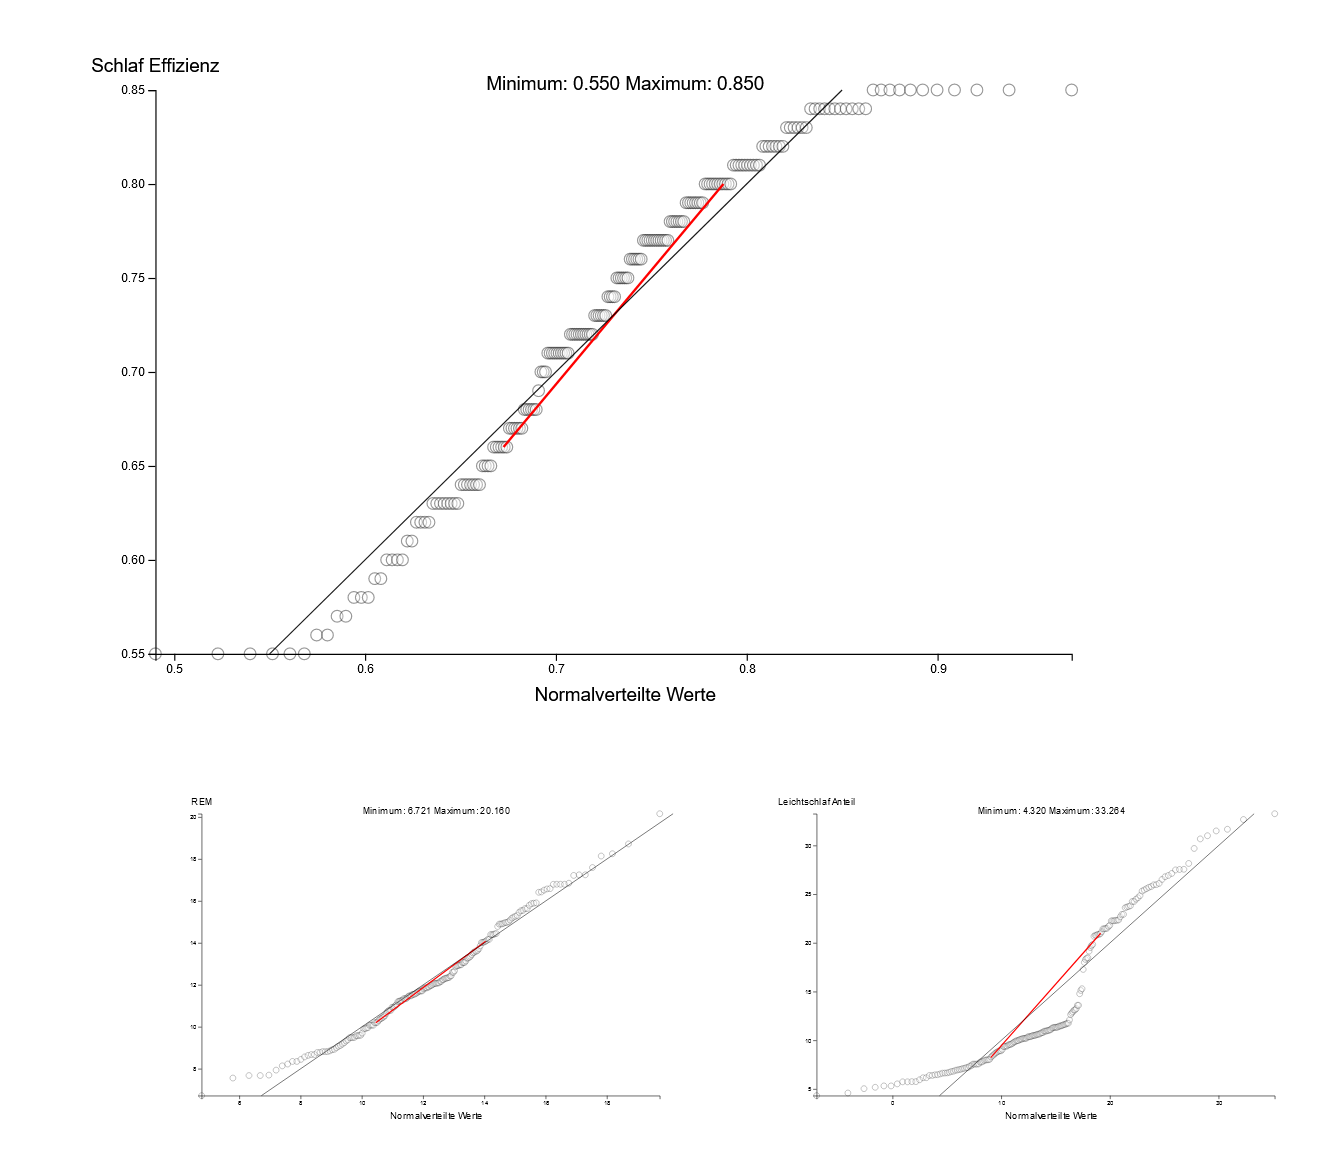
\includegraphics [width = 0.8\textwidth]{Bsp_QQ-Plot.JPG}
  \caption{Visualisierung Eins: Anwendungsbeispiel}
\end{figure}

\subsection{Anwendung Visualisierung Zwei}

Im zweiten Schritt der visualisierung wurden die Attribute REM und Leichtschalf Anteil untersucht. Man kann gut erkennen, dass es eine Zusammenhang zwischen niedrigem Leichtenschlaf und hoher Schlafeffizienz gibt. Bei hohem leichtschlaf Anteil geht ein leichtes Cluster zu einer reduzierten Schlafeffizienz. 
Der zusammenhang zwische REM und Schlafeffizienz, besteht aus parallel Absenkenden Strichen, dies deutet darauf hin, dass mit Anstieg des REM Schlafanteils die Schlaff Effizienz abnimmt.

\begin{figure}[h]

  \centering
  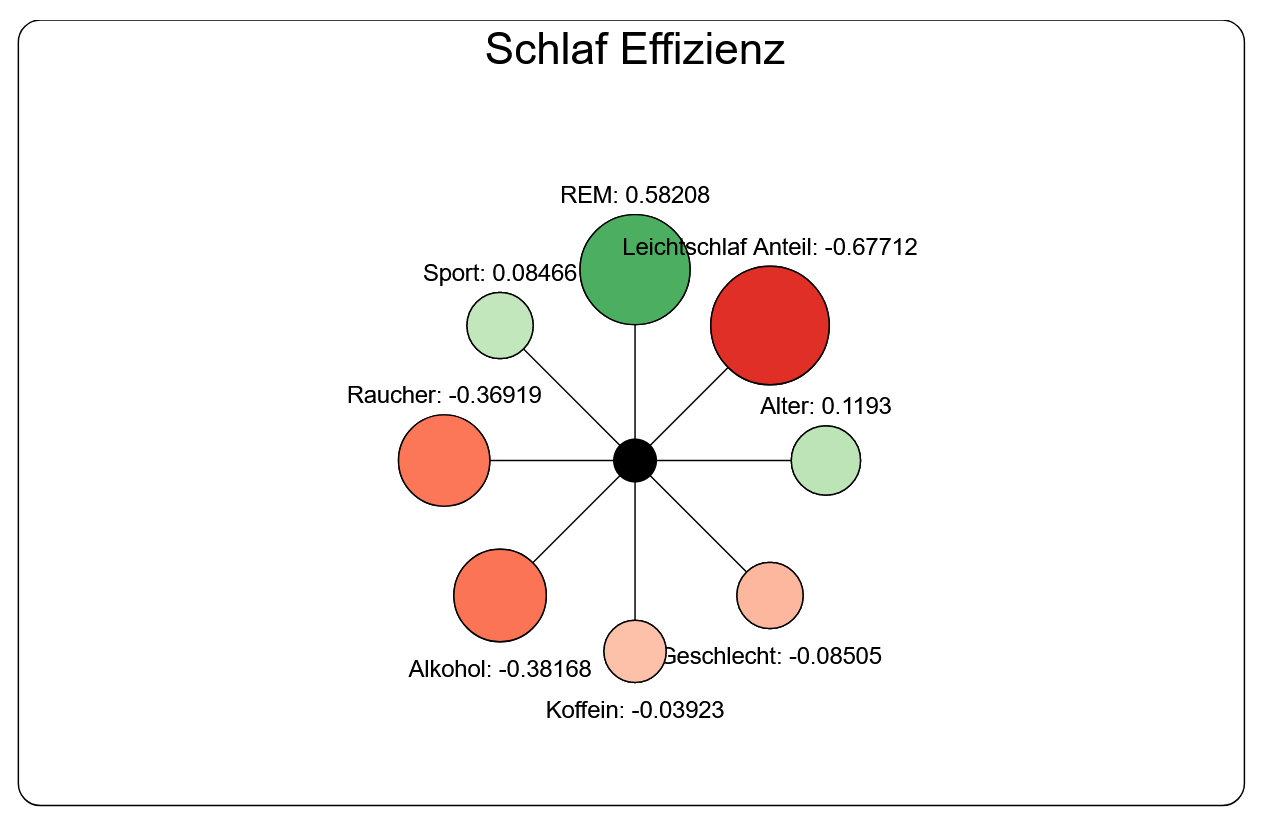
\includegraphics [width = 0.8\textwidth]{Bsp_ImpactGraph.PNG}
  \caption{Visualisierung Eins: Anwendungsbeispiel}

  
\end{figure}

So lässt sich nur aus der Visualisierung ohne Vorwissen die Hypothese entwickeln, dass mit geringerer Schlafeffizienz die REM Schlafanteile sinken und der Anteil des leichten Schlafes erhöht wird.

\subsection{Anwendung Visualisierung Drei}

Die durch Visualisierung 2 entwicklete Hypothese, kann durch Visualisierung 3 unterstützt werden. 
Die Repräsentation der Korrelierung durch die Kugeln  in größe und Farbe zeigen stützen, dass die Korrelation von REM auf die Schlaffeffizienz positiv ist und die korrelation des Leichtschlafanteils negativ. 
Weiter kann man erkennen, dass die Standardmäßig angezeigten Verhaltensweisens Attribute mit der Schlafeffizienz korrelieren. 


\section{Verwandte Arbeiten}
Führen sie eine kurze Literatursuche in der wissenschaftlichen Literatur zu Informationsvisualisierung und Visual Analytics nach ähnlichen Anwendungen durch. Diskutieren sie mindestens zwei Artikel. Stellen sie Gemeinsamkeiten und Unterschiede dar.

\section{Zusammenfassung und Ausblick}
Fassen sie die Beiträge ihre Visualisierungsanwendung zusammen. Wo bietet sie für die Personen der Zielgruppe einen echten Mehrwert.

Was wären mögliche sinnvolle Erweiterungen, entweder auf der Ebene der Visualisierungen und/oder auf der Datenebene?

\section*{Anhang: Git-Historie}

\printbibliography

\end{document}

